\renewcommand{\(}{\left(}
\renewcommand{\)}{\right)}
\chapter{Equidistant spiral sampling}
\section{Introduction}
We want to illuminate different points in the back focal plane of a
micro objective. Its convenient to have a 1D indexing scheme for these
points. Due to the circular symmetry a spiral sampling [1983Ahn] comes
to mind. 

\section{Archimedes Spiral}
An Archimedes spiral in polar coordinates $(r,\theta)$ is defined like
this:
\begin{align} \label{eqn:def}
  r(\theta)=a\,\theta.
\end{align}
The step height $h$ of the spiral is given by
\begin{align}
  h=\abs{r(\theta)-r(\theta+2\pi)}=r(2\pi)=2\pi a.
\end{align}
\section{Equidistance sampling}
We want to start sampling in the center at $r(0)=0$ and sample the arc
length of the spiral with equidistant points. The arc length of an
archimedes spiral is [Weisstein]:
\begin{align} \label{eqn:arclength}
  s(\theta)=\frac{a}{2}\(p\,\theta + \log(p\,\theta)\)\quad\textrm{with}\quad
  p=\sqrt{1+\theta^2}.
\end{align}
The arc length $\Delta s$ between successive points along the spiral
should be equal to the step height $h$. Starting from the central
point $\theta_0=0$ the arc length where to sample the $i-$th point can
be obtained by inverting equation \eqref{eqn:arclength}:
\begin{align}
  \theta_i=\theta(i\,\Delta s).
\end{align}
This inversion can be done efficiently with Newton interation
[Wikipedia]:
\begin{align}
  x_0&=1,\\
  x_{n+1}&=x_n-\frac{f(x)}{f'(x)}.
\end{align}
Here we introduce the function $f(\theta)$ that vanishes at a given arc
length $s$ and its derivative $f'(\theta)$:
\begin{align}
  \label{eqn:f}
  f(\theta)&=\frac{a}{2}\(p\,\theta+\log(p\,\theta)\)-s,\\
  f'(\theta)&=\frac{\partial f(\theta)}{\partial \theta}=
  \frac{a}{2}\frac{(1+2\theta^2)(1+p\theta)}{p^2 \theta}.
\end{align}
\section{Filling the back focal plane}
We want to find the coordinates of equaly distributed sampling points
along the arc length inside of a circle with radius R. We put the
first sampling point $\theta_0=0$ in the center and the last point
$\theta_n$ on the periphery of the circle. By definition
\eqref{eqn:def} of the spiral we know
\begin{align}
  \theta_n=R/a.
\end{align}
Now we obtain the arc length $s(\theta_n)$ of the spiral contained
inside the circle via \eqref{eqn:arclength}. Dividing by the number of
sub-intervals gives the apropriate sampling step $\Delta s =
s(\theta_n)/(n-1)$.

Note that we are only interested in solutions with $\Delta s=h$. We
want the sampling step to be equal to the step height $h=2\pi a$ of
the spiral. We therefore need to find the zero of the function:
\begin{align} \label{eqn:g}
  g(a)&=\frac{s(\theta_n)}{n-1}-2\pi a\\
  &=\frac{a}{2}\frac{p\theta_n+\log p\theta_n}{n-1}-2\pi a\\
  &=\frac{a}{2}\frac{\sqrt{1+\frac{R^2}{a^2}}\frac{R}{a}+
    \log\(\sqrt{1+\frac{R^2}{a^2}}\frac{R}{a}\)}{n-1}-2\pi a.
\end{align}
Actually we know $a\not =0$ so we can transform the function to
simplify its derivative:
\begin{align} \label{eqn:g1}
  g_1(a)&=\underbrace{\sqrt{1+\frac{R^2}{a^2}}}_{p_1}\frac{R}{a} 
  +\log\(\sqrt{1+\frac{R^2}{a^2}}\frac{R}{a}\)-4\pi (n-1),\\
  g_1'(a)&=-\frac{R^3}{p_1}\frac{1}{a^4}-\frac{R^2}{p_1^2}\frac{1}{a^3}-R
    p_1\frac{1}{a^2}-\frac{1}{a}.
\end{align}
The Newton method can be used to find the zero $a_0$ of $g(a)$. Then
$\Delta s$ can be obtained and the circle drawn.

% for i in *.pgm ; do potrace $i ;done
\begin{figure}[h]
  \begin{center}
    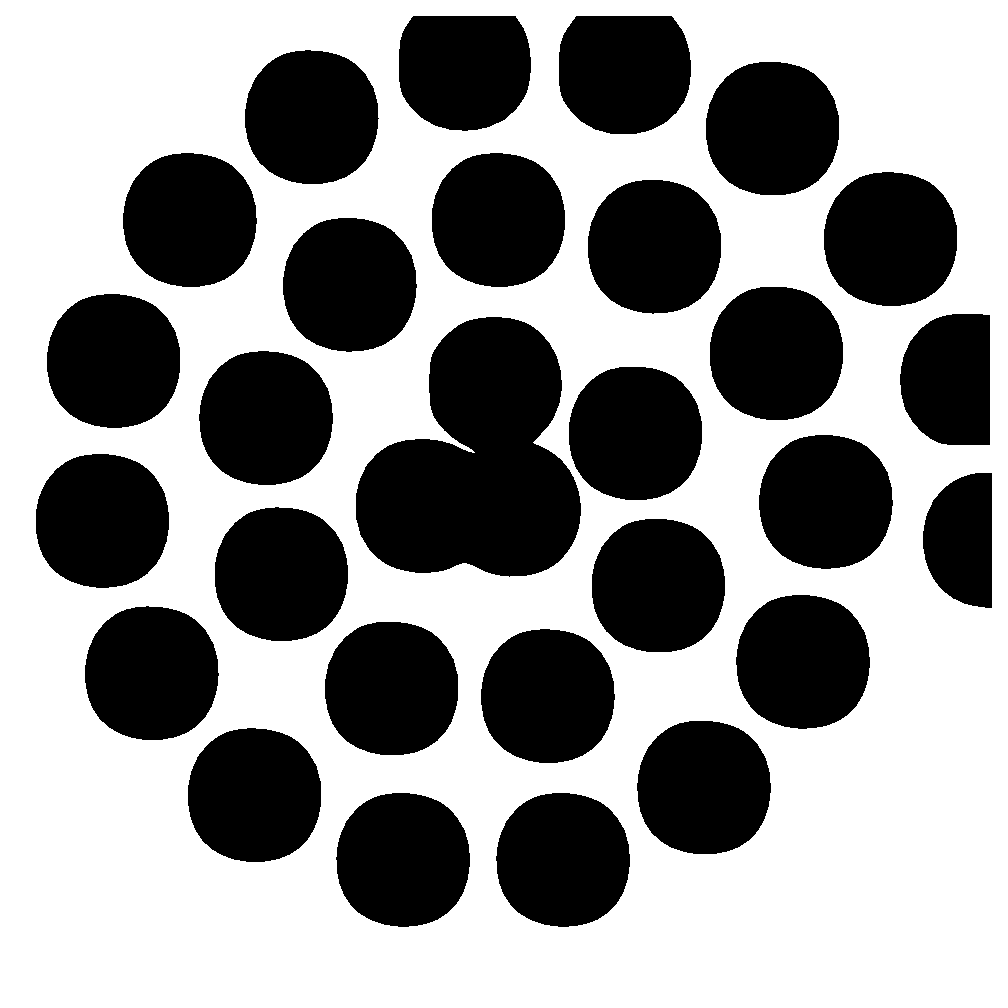
\includegraphics[width=.3\columnwidth]{../app_spiral/o0030}
    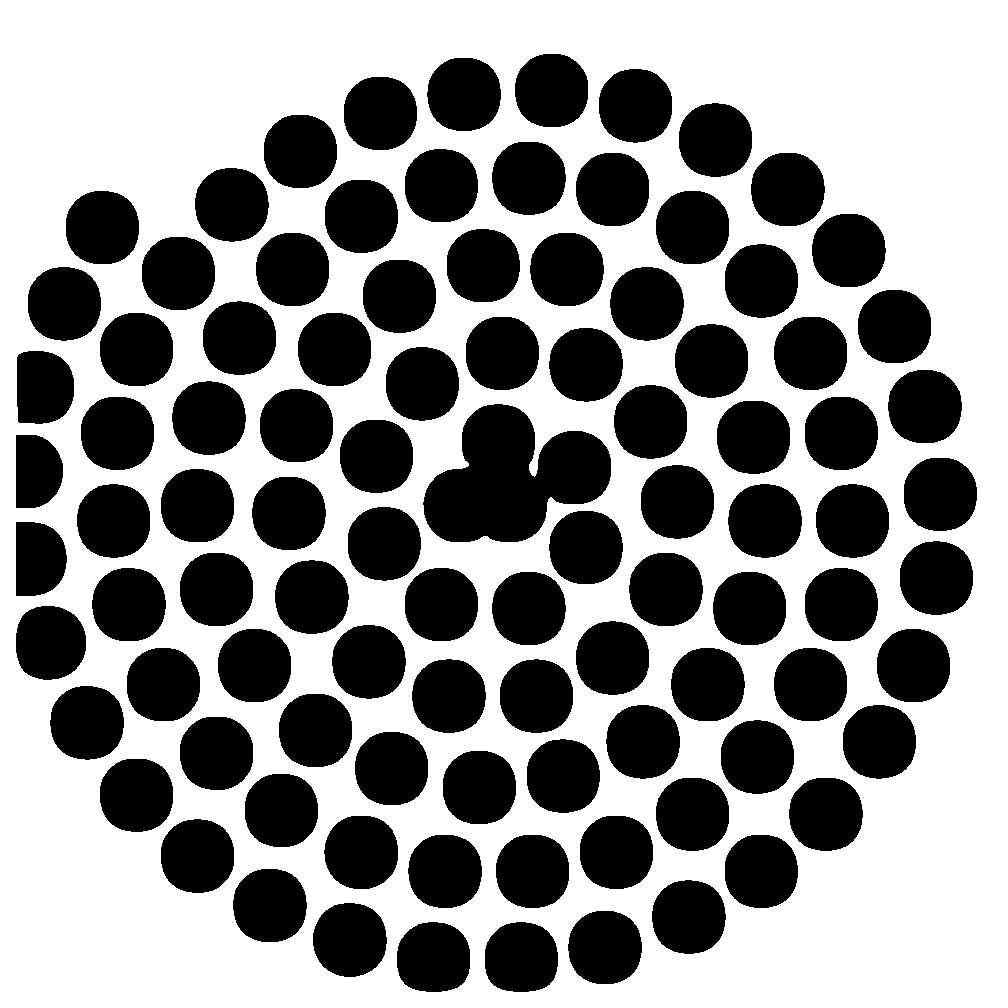
\includegraphics[width=.3\columnwidth]{../app_spiral/o0100}
    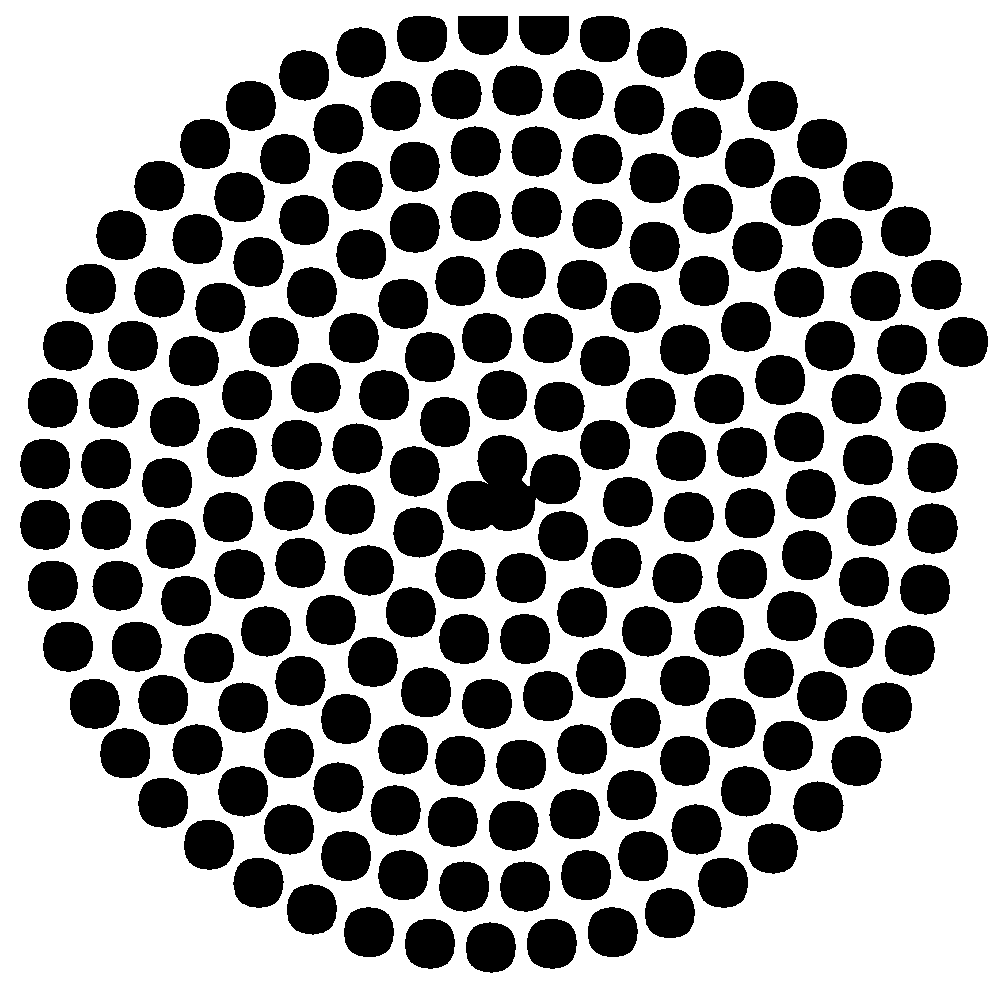
\includegraphics[width=.3\columnwidth]{../app_spiral/o0200}
    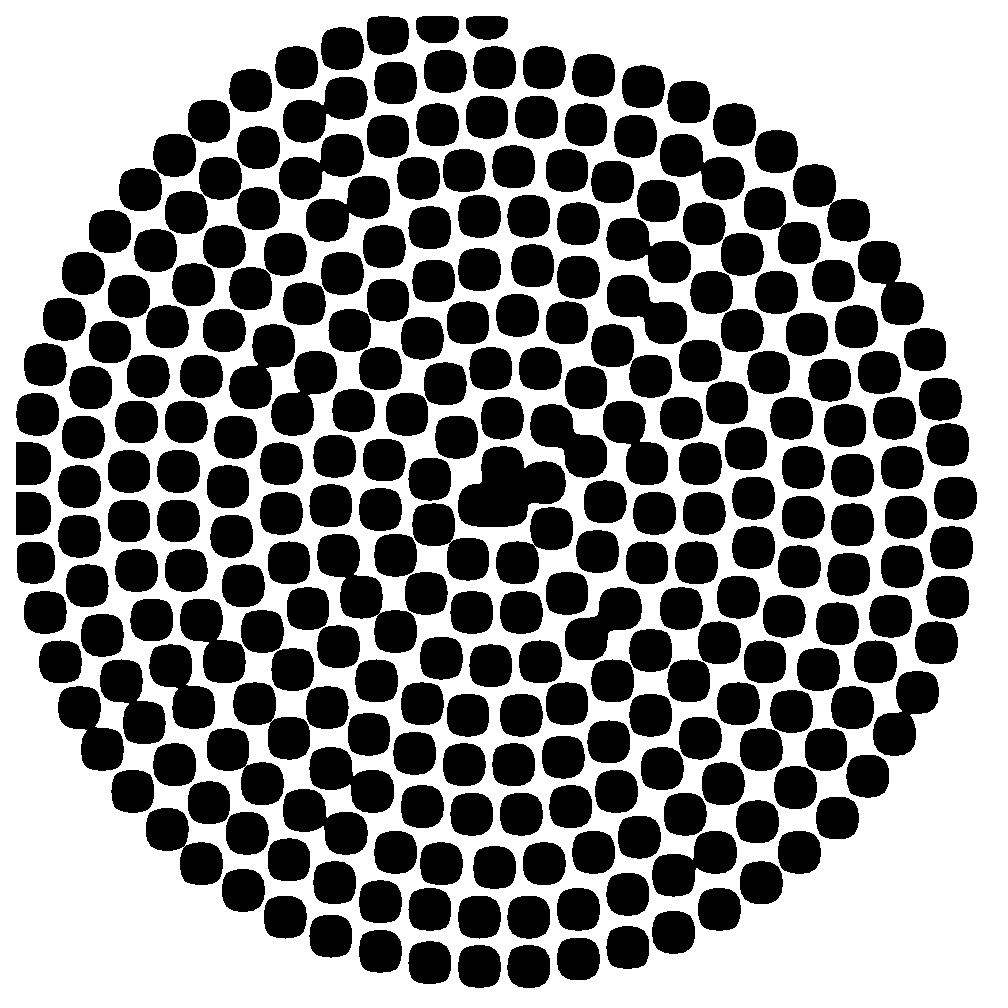
\includegraphics[width=.3\columnwidth]{../app_spiral/o0300}
    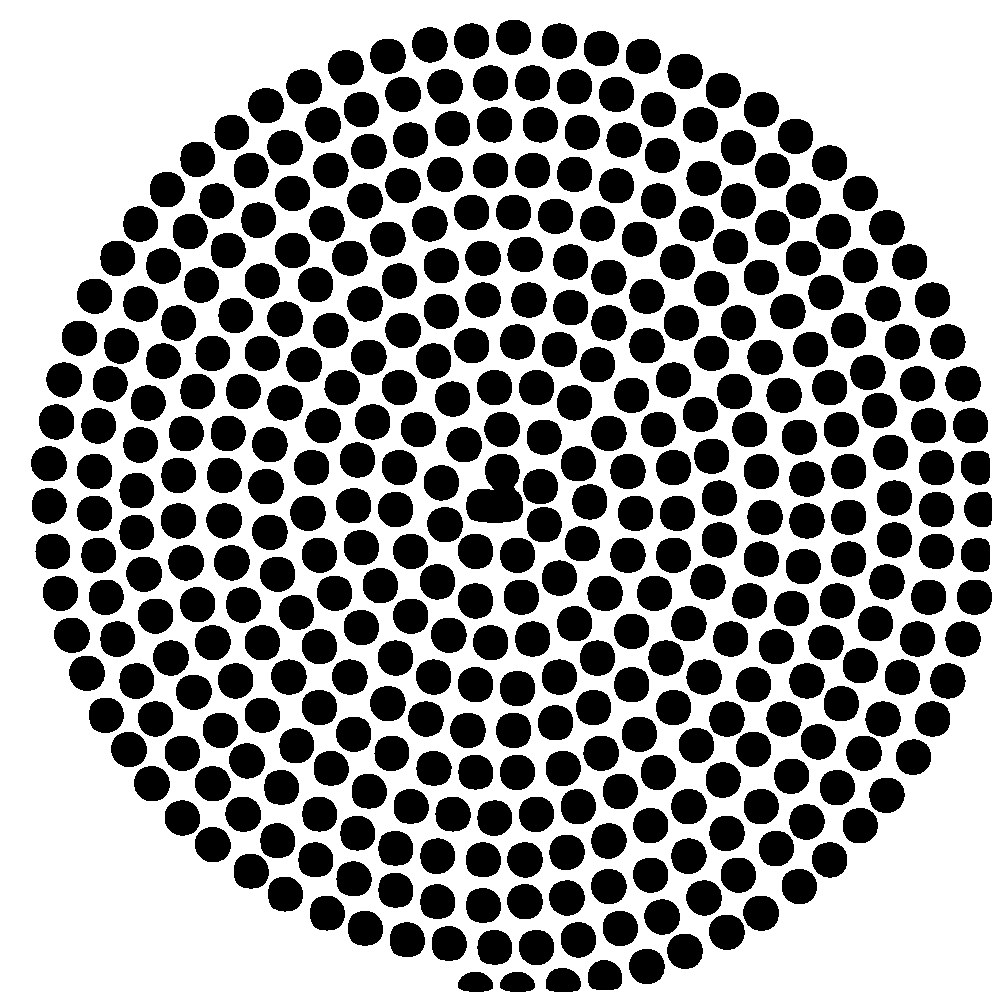
\includegraphics[width=.3\columnwidth]{../app_spiral/o0400}
    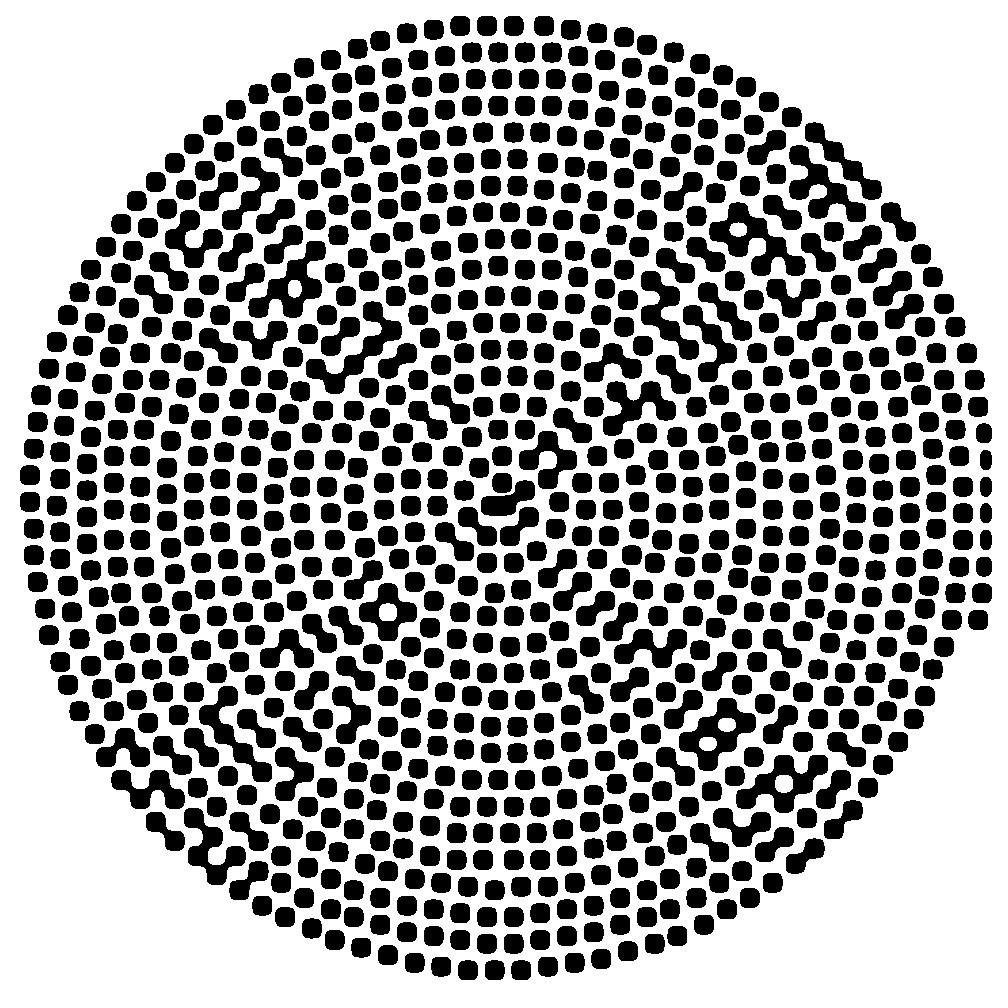
\includegraphics[width=.3\columnwidth]{../app_spiral/o1024}
  \end{center}
  \caption{Equidistant sampling of a circle of the same radius
    $R=128$ with different number of points (from top left to bottom
    right: 30, 100, 200, 300, 400, 1024).}
\end{figure}

\section{Improvement for sampling with disks}
It is useful to modify the filling formula \eqref{eqn:g} such, that
disks with radius $r_s=\alpha\Delta s/2$ on the sample points don't
overlap the periphery of the big circle. Again we have $\theta_n=R/a$ but $R$ is smaller than the back focal plane radius $R_B$:
\begin{align}
  R=R_B-r_s.
\end{align}
Thus we can define the equivalent to \eqref{eqn:g1}:
\begin{align}
  \begin{split}
  g_2(a)&=\overbrace{\sqrt{1+\frac{(R_B-\pi\alpha a)^2}{a^2}}}^{p_2}
  \frac{R_B-\pi\alpha a}{a}+
  \log\(\sqrt{1+\frac{(R_B-\pi\alpha a)^2}{a^2}}\frac{R_B-\pi\alpha a}{a}\)\\ 
  &-4\pi (n-1),\end{split}\\
  g_2'(a)&=
  -\frac{R^3}{p_2}\frac{1}{a^4}
  -\(\frac{\pi\alpha R^2}{p_2}+\frac{R^2}{p_2^2}\)\frac{1}{a^3}
  -\(R p_2+\frac{\pi\alpha R}{p_2^2}\)\frac{1}{a^2}-\(\pi\alpha p_2+1\)\frac{1}{a}+\frac{\pi\alpha}{R}.
\end{align}


\begin{figure}[h]
  \begin{center}
    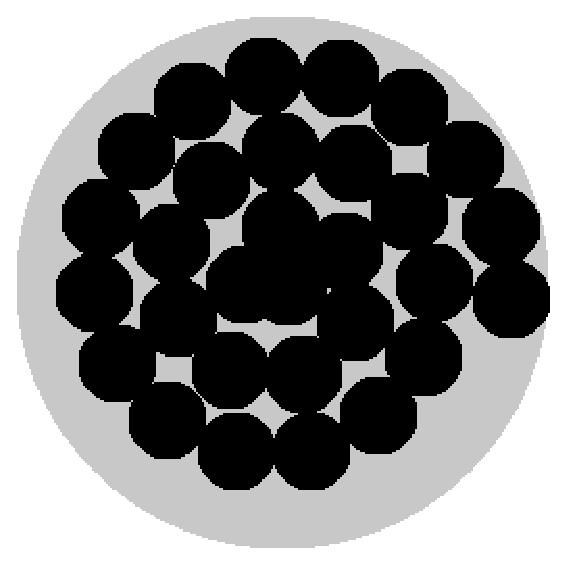
\includegraphics[width=.3\columnwidth]{../app_spiral/q0030}
    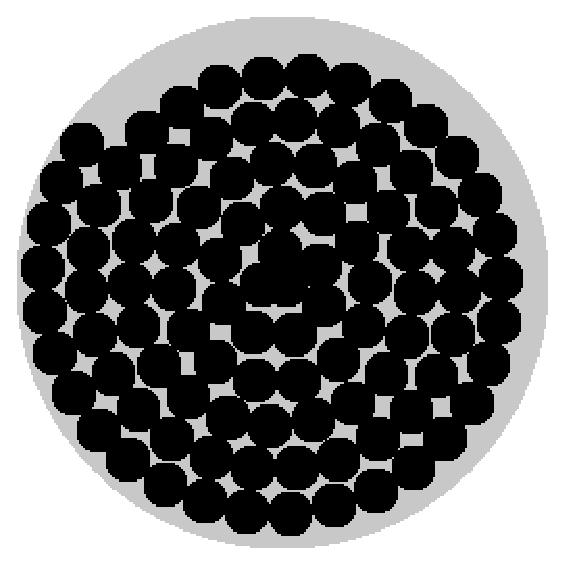
\includegraphics[width=.3\columnwidth]{../app_spiral/q0100}
    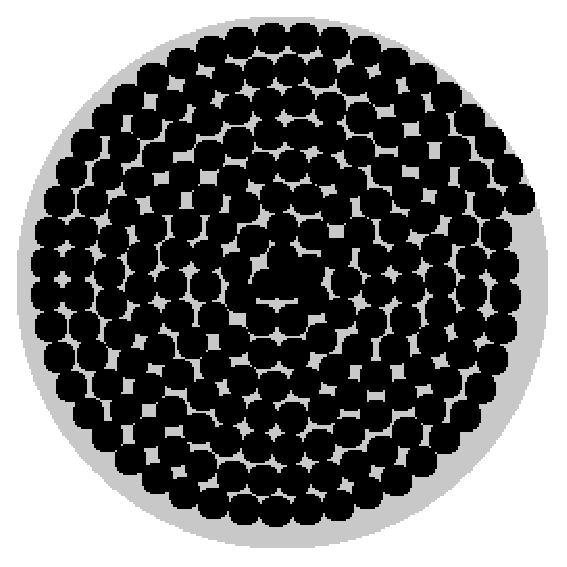
\includegraphics[width=.3\columnwidth]{../app_spiral/q0200}
    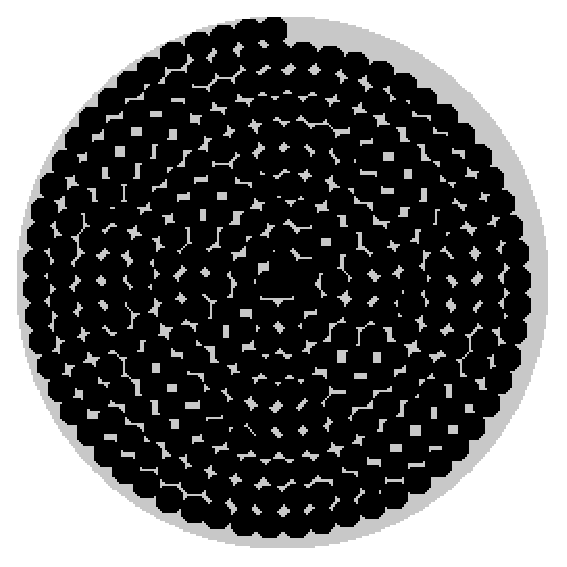
\includegraphics[width=.3\columnwidth]{../app_spiral/q0300}
    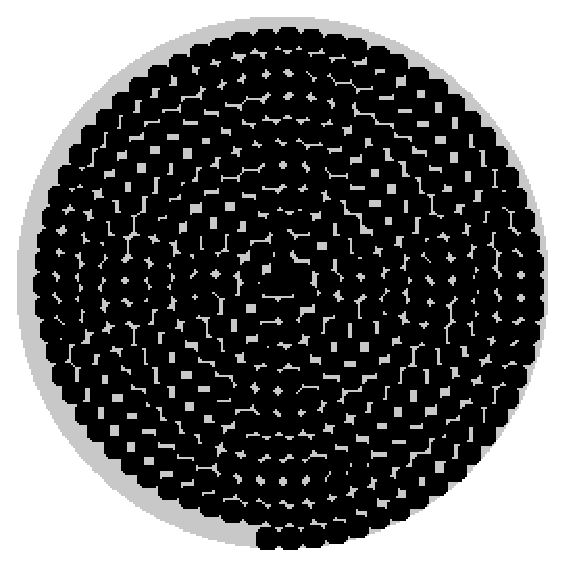
\includegraphics[width=.3\columnwidth]{../app_spiral/q0400}
    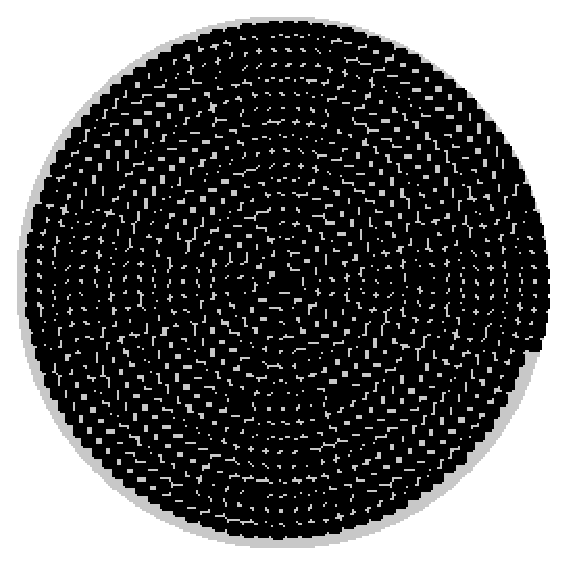
\includegraphics[width=.3\columnwidth]{../app_spiral/q1024}
  \end{center}
  \caption{A back focal plane of radius 100 is filled with equidistant
    spiral sampling, ensuring that the outermost disk is contained
    inside. The number of disks are (from top left to bottom right):
    30, 100, 200, 300, 400, 1024.}
\end{figure}

%% FindRoot[{a x == R, a/2 (Sqrt[1+x^2]x+Log[Sqrt[1+x^2]x]) == n * 2 pi a + R/a}, {{x, 1}, {a, 1}}]

%% @ARTICLE{4307732,
%% author={Ahn, C. B. and Kim, J. H. and Cho, Z. H.},
%% journal={Medical Imaging, IEEE Transactions on}, title={High-Speed Spiral-Scan Echo Planar NMR Imaging-I},
%% year={1986},
%% month={mar.},
%% volume={5},
%% number={1},
%% pages={2 -7},
%% keywords={},
%% doi={10.1109/TMI.1986.4307732},
%% ISSN={0278-0062},}

%% Weisstein, Eric W. "Archimedes' Spiral." From MathWorld--A Wolfram
%% Web Resource. http://mathworld.wolfram.com/ArchimedesSpiral.html


%% http://en.wikipedia.org/wiki/Newton's_method

%% multidimensional newton method
%% http://math.fullerton.edu/mathews/n2003/NewtonSystemMod.html
